\chapter{Introduction}
\label{chap:intro}
\section{VLSI Design Flow}
The development cycle of any digital IC is governed by a few fundmanetal steps or processes that are sequentially followed. The first step begins with designing an algorithm to solve the problem and meet the requirements. Coming up with an algorithm is followed by designing an architecture which can be realized on hardware that is feasible in the desired resource-constrained use case. Different architectures can be proposed for the same algorithm which can be further optimized at the gate level. As shown in the figure \ref{fig:vlsi}, in order to fully exploit the benefit of having an ASIC design, after the gate level modelling, transistor level optimizations are also important. The last stage of the design cycle ends with modifications at the device level.

A small modification at an earlier level in the design flow can lead to a significant change at a later level. A single multiplier that could be eliminated at the architectural level would lead to saving thousands of transistors indicating the significance of higher level optimizations. Since the effects of an optimization are reflected in the following stages, it is essential to fully explore the various possible models or designs.

\begin{figure}[h]
\label{fig:vlsi}
	\caption{VLSI Design Flow}    
    \centering
    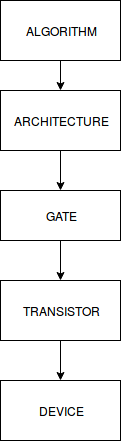
\includegraphics[width=0.1\textwidth]{vlsi_dESIGN}
\end{figure}

\section{Machine Learning}
The field of machine learning is not one that is new. These algorithms have been in existence for a long time although only in recent years they have come into popularity, especially neural networks and deep learning, thanks to the rapid increase in computational power. The GPU has aided in increasing the scale of these models to actually work effectively on real-world tasks. While major strides have been made in improving these algorithms by extensive training and refinement at an algorithmic level, research into architectural changes has been limited. \\
Due to recent advancements in compute power in embedded/mobile device, there is now a possibility of implementing these computationally expensive models on devices with a tighter power, memory and compute constraint than was previously there on non-mobile devices. \\
Indicative of the growing interest in embedded implementations of such networks, in the last couple of years there have been some works on FPGA deployment of LSTMs but none of them seem to leveraging the VLSI digital signal processing techniques for optimization.% [refs to these works] 
VLSI DSP techniques such as systolic arrays, unfolding, distributed arithmetic, CORDIC, pipelining etc., have been in use for the past 30 years for the fields of communication, filters, image processing lend themselves really well for machine learning algorithms as well. Recent work inspired by these techniques optimize Support Vector Machines and Convolutional Neural Networks.%[refs to Rafis papers] 
One branch of neural networks that is explicitly suited for tasks that are applicable in mobile devices are Recurrent Neural Networks. These networks are suited for data that is sequential in nature and have been shown to be effective at tasks such as handwriting recognition and generation, speech and speaker recognition, language modelling, speech synthesis to name a few. \\

\section{Literature Review}
A specialised version of the RNN that is extremely popular for commercial application is the Long Short Term Memory network (LSTM). It is adept at establishing long term dependencies in data . As of 2016, many software giants such as Google, Apple and Microsoft had LSTMs as a fundamental unit in their products. Google incorporated LSTMs for the speech recognition task on the handheld device and also into their smart assistant as well as Google Translate. \\
\\
The typical computational power required by LSTMs is demanding. The challenge of deploying these models is further increased due to the size of the models themselves which needs to be stored locally to fully execute these tasks. 

-original paper
-lstm odyssey
-compression papers
-no proper application of VLSI DSP in this field. can lead to significant improvement to help deploy on devices.

\section{Problem Formulation}
Our goal is to leverage both the best of the available algorithmic optimizations or a combination of those followed by VLSI DSP techniques that are suited to exploit some unique properties of LSTM.
% change to third person
We will first go through the preliminaries that establish the algorithm of Long Short Term Memory Networks. We will then systematically go through the different levels of optimization, from algorithmic to an architectural level, that can be applied to these networks.
